%\section{Photon Detection System (PDS) Overview}
%%%%%%%%%%%%%%%%%%%%%%%%%%%%%%%%%%%%%%%%%%%%%%%%%%%%
\newcommand{\tzero}{\ensuremath{t_0}\xspace}

\section{Introduction} % Anne
\label{sec:fdsp-pd-intro}
%\metainfo{\color{blue} Content: Segreto, Warner, Wilson}

The \dword{dune} \dword{fd} consists of detector systems for charge and light produced by an ionization event in the \dword{lartpc}.  The charge detection system permits both calorimetry and position determination, with two of the three spatial coordinates ($y$ and $z$)  established by the position of the \dword{apa} wires receiving the charge and the third ($x$) by the arrival time of the charge.  Locating the $x$ position requires independently determining the time of the ionization event, a clock start time.  Two systems provide this in \dword{dune}:  the \dshort{fnal} accelerator system for neutrino beam related events and the \dword{pds}.  

Neutrino \dword{cpv} and other elements of the \dword{dune} long-baseline neutrino program are possible without data from the \dword{pds}.  The neutrino beam timing allows full functionality of the \dword{apa}s, and the deep underground location reduces the possibility of in-time background events from cosmic rays and other sources to a negligible level.  
Similarly, \dword{dune} can detect \dwords{snb} originating within the galaxy without the \dword{pds} because the presence of thousands of low-energy neutrino events, even if they consist only of few millimeter long tracks, provides an unambiguous signal in the \dword{tpc}.
By contrast, \dword{dune}'s nucleon decay physics cannot be executed without the \dword{pds}.  The inability to establish a clock start time (\tzero) makes it impossible to determine whether a candidate proton decay event was fully contained in the detector volume or associated with objects entering the detector from the outside.  Determining \tzero also allows the energy reconstructed by the \dword{tpc} to be corrected for charge lost due to electron capture and other transport effects in the \dword{tpc}. This physics sets the requirement on minimum light yield in the dimmest regions of the detector far from the photon detectors %(SP-FD-3) 
and timing resolution, %(SP-FD-4), 
described further in Appendix Section~\ref{subsec:fdsp-pd-simphys-ndk}.

While only absolutely required for proton decay searches, the \dword{pds} directly enhances physics capabilities for all three \dword{dune} physics drivers, opens up prospects for further physics explorations, and contributes to a more robust set of operating points of the detector that help all physics.   For \dword{snb} neutrino events, the \dword{pds} allows proper location of the event vertex, and improves energy resolution by allowing position-dependent energy corrections and complementary direct calorimetric measurements, 
improving energy resolution and possibly sensitivity to underlying supernova dynamical models.  The \dword{pds} also enables a complementary triggering scheme for the burst itself, increasing 
reliability, reducing dead time, and extending the sensitivity further out to nearby dwarf galaxies (see Appendix Section~\ref{subsec:fdsp-pd-simphys-snb}). Applications to supernova physics set the average light yield requirement. % (SP-FD-3).


The \dword{pds} can also measure energy calorimetrically for all classes of events, working as a crosscheck of the energy measured by the \dword{tpc} or improving the resolution when both measurements are used together (see Appendix Section~\ref{subsec:fdsp-pd-simphys-beam}).  In the event that the \dword{dune} \dword{tpc} cannot operate at its goal electric field of \SI{500}{V/cm}, the \dword{pds} energy measurements could compensate for reduced charge detector performance because light production increases relative to the free charge for lower \efield{}.

The \dword{pds} could open new areas of investigation.  The few-MeV scale solar neutrino interactions occur as isolated events in time and space.  Suppressing radiological and noise related backgrounds to pull out a signal for these events likely requires redundant measurements with charge and light.  The \dword{pds} may also provide a means for identifying events with Michel electrons produced from the decay of a stopped muon. Tagging these electrons can be used to estimate the antineutrino content of the beam flux or further reduce nucleon decay backgrounds (see Appendix Section~\ref{subsec:fdsp-pd-simphys-beam}).
 
%The remaining sections further develop the specification and design of a \dword{pds} that supports \dword{dune} physics.

Volume~\volnumberphysics{}, \voltitlephysics{},  of this \dword{tdr} describes the detailed physics simulations of the main \dword{dune} physics drivers.  
The \dword{pds} performance specifications have been established and validated in part by simulation.  Details of this simulation, which includes non-uniformity in light yield due to the optical properties of the argon, electronics response, and realistic reconstruction, are presented in Appendix Section~\ref{sec:fdsp-pd-simphys}.


\section{Design Specifications and Scope}
\label{sec:pds:des-specs}
% Source document for the tables is docDB 6422 \dword{dune} Far Detector Single Phase Photon Detector
\subsection{Specifications}
Based on the physics drivers and additional simulation studies described in Appendix Section~\ref{sec:fdsp-pd-simphys}, Table~\ref{tab:specs:SP-PDS} summarizes the \dword{pds} specifications necessary to achieve the \dword{dune} science objectives. 
In the remainder of this chapter, we present a design that meets or exceeds the specifications. Section~\ref{sec:fdsp-pd-validation} summarizes an extensive set of prototypes that validate the assumptions used in the design.

\cleardoublepage
% This file is generated, any edits may be lost.

\begin{longtable}{p{0.14\textwidth}p{0.13\textwidth}p{0.18\textwidth}p{0.22\textwidth}p{0.20\textwidth}}
\caption{Specifications for SP-PDS \fixmehl{ref \texttt{tab:spec:SP-PDS}}} \\
  \rowcolor{dunesky}
       Label & Description  & Specification \newline (Goal) & Rationale & Validation \\  \colhline

   \newtag{SP-FD-1}{ spec:min-drift-field }  & Minimum drift field  &  $>$\,\SI{250}{ V/cm} \newline ( $>\,\SI{500}{ V/cm}$ ) &  Lessens impacts of $e^-$-Ar recombination, $e^-$ lifetime, $e^-$ diffusion and space charge. &  ProtoDUNE \\ \colhline
    
   
  \newtag{SP-FD-2}{ spec:system-noise }  & System noise  &  $<\,\SI{1000}\,e^-$ &  Provides $>$5:1 S/N on induction planes for  pattern recognition and two-track separation. &  ProtoDUNE and simulation \\ \colhline
    
   
  \newtag{SP-FD-3}{ spec:light-yield }  & Light yield  &  $>\,\SI{20}{PE/MeV}$ (avg), $>\,\SI{0.5}{PE/MeV}$ (min) &  Gives PDS energy resolution comparable that of the TPC for 5-7 MeV SN $\nu$s, and allows tagging of $>\,\SI{99}{\%}$ of nucleon decay backgrounds with light at all points in detector. &  Supernova and nucleon decay events in the FD with full simulation and reconstruction. \\ \colhline
    
    \\ \rowcolor{dunesky} \newtag{SP-FD-4}{ spec:time-resolution-pds } & Name: Time resolution \\
    Description & The time resolution of the photon detection system shall be less than 1 microsecond in order to assign a unique event time.   \\  \colhline
    Specification (Goal) &  $<\,\SI{1}{\micro\second}$  ( $<\,\SI{100}{\nano\second}$ ) \\   \colhline
    Rationale &   Enables \SI{1}{mm} position resolution for \SI{10}{MeV} SNB candidate events for instantaneous rate $<\,\SI{1}{m^{-3}ms^{-1}}$.  \\ \colhline
    Validation &   \\
   \colhline

   \newtag{SP-FD-5}{ spec:lar-purity }  & Liquid argon purity  &  $<$\,\SI{100}{ppt} \newline ($<\,\SI{30}{ppt}$) &  Provides $>$5:1 S/N on induction planes for  pattern recognition and two-track separation. &  Purity monitors and cosmic ray tracks \\ \colhline
    
    \\ \rowcolor{dunesky} \newtag{SP-FD-15}{ spec:lar-n-contamination } & Name: LAr nitrogen contamination \\
    Description & The nitrogen contamination in the LAr shall remain below 25 ppm in order not to significantly affect the number of photons that reach the detectors (for both fast and late light components).   \\  \colhline
    Specification &  $<\,\SI{25}{ppm}$ \\   \colhline
    Rationale &   Maintain \SI{0.5}{PE/MeV} PDS sensitivity required for triggering proton decay near cathode.  \\ \colhline
    Validation & In situ measurment  \\
   \colhline


    \\ \rowcolor{dunesky} \newtag{SP-PDS-1}{ spec:ly-uniformity } & Name: Light yield uniformity within the active volume. \\
    Description & The light yield in even the dimmest regions of the detector shall be sufficient to correctly associate scintillation light with events with energy > 200 MeV with efficiency >\SI{99}{\%}. The goal is to dramatically improve the uniformity to improve background rejection, triggering efficiency, and energy resolution.   \\  \colhline
    Specification (Goal) &  $>\,\SI{0.5}{pe/MeV}$  ( >\SI{4}{pe/MeV} ) \\   \colhline
    Rationale &   Fiducializing nucleon decay backgrounds with  $>\,\SI{99}{\%}$ efficiency at all points in the detector.  \\ \colhline
    Validation & Simulated nucleon decay events in the far detector.  \\
   \colhline

    \\ \rowcolor{dunesky} \newtag{SP-PDS-2}{ spec:spatial-localization } & Name: Spatial localization \\
    Description & Events inside the active volume shall be localized in the Y-Z plane  to within < \SI{2.5}{\meter} using light signals.   \\  \colhline
    Specification &  < \SI{2.5}{\meter} \\   \colhline
    Rationale &   Enables more accurate matching of photon detector and TPC signals.  \\ \colhline
    Validation & Supernova neutrino and nucleon decay simulation in the far detector.  \\
   \colhline

    
   
  \newtag{SP-PDS-3}{ spec:env-light-exposure }  & Environmental light exposure  &  \num{0} sunlight.  All other unfiltered sources: $<\,\num{30}$ minutes integrated across all exposures &  Prevent damage to wavelength-shifting coatings due to UV exposure &  ProtoDUNE, IU studies \\ \colhline
    
    \\ \rowcolor{dunesky} \newtag{SP-PDS-4}{ spec:env-humidity-limit } & Name: Environmental humidity limit \\
    Description & All working environments with exposed TPB coatings must maintain <\SI{50}{\%} Relative Humidity (RH) at  \SI{70}{\degree F}.   \\  \colhline
    Specification (Goal) &  < \SI{50}{\%} RH at \SI{70}{\degree F}  ( ALARA ) \\   \colhline
    Rationale &     \\ \colhline
    Validation &   \\
   \colhline

   
  \newtag{SP-PDS-5}{ spec:light-tightness }  & Light-tight cryostat  &  Cryostat light leaks responsible for $<\,\SI{10}{\%}$  of data transferred from PDS to DAQ &  Minimizing false triggers due to cryostat light leaks helps limit the data transfer rate to  \dshort{daq}. &  \dshort{pdsp} and \dshort{iceberg} \\ \colhline
    
   
  \newtag{SP-PDS-6}{ spec:ed-light }  & Light from electrical discharge  &  Light generated by HV system responsible for $<\,\SI{10}{\%}$ total trigger rate in DAQ &  Minimizing false triggers due to corona light from \dword{hv} discharge helps limit the data transfer rate to the \dword{daq}. &  \dword{pdsp} and \dword{iceberg} \\ \colhline
    
    \\ \rowcolor{dunesky} \newtag{SP-PDS-7}{ spec:mech-deflection } & Name: Mechanical deflection (static) \\
    Description & The PDS shall not deviate more than 5mm from nominal position in any APA orientation due to PD load   \\  \colhline
    Specification &  $<\,\SI{5}{\milli\meter}$ \\   \colhline
    Rationale &   Constrain PD motion (static and dynamic load) to avoid damaging APA  \\ \colhline
    Validation & PD FEA, ProtoDUNE, ICEBERG, Ash River integration tests, CERN pre-production integration test  \\
   \colhline

    \\ \rowcolor{dunesky} \newtag{SP-PDS-8}{ spec:apa-install } & Name: Clearance for installation through APA side tubes \\
    Description & PD modules must fit and be secured to the APA through slots in one side of the APA, as designed in concert with APA group.   \\  \colhline
    Specification &  $>$\SI{1}{\milli\meter} \\   \colhline
    Rationale &     \\ \colhline
    Validation &   \\
   \colhline

   
  \newtag{SP-PDS-9}{ spec:mech-compatibility }  & No mechanical interference with APA, SP-CE and SP-HV detector elements (clearance)  &  $>\,\SI{1}{\milli\meter}$ &  PD mounting and securing element tolerances must prevent interference with APA and CE cable bundles. &  Validation will occur in \dword{iceberg}, Ash River integration  tests, and the \dword{cern} pre-production integration tests. \\ \colhline
    
   
  \newtag{SP-PDS-10}{ spec:pds-cable }  & APA intrusion limit for PD cable routing   &  $<\,\SI{6}{\milli\meter}$ &  \dword{pd} modules must install into \dword{apa} frames following wire wrapping.  \dword{pd} modules must not occlude \dword{apa} side tubes. &  \dword{iceberg}, Ash River integration  tests, and the CERN pre-production integration tests \\ \colhline
    
   
  \newtag{SP-PDS-11}{ spec:pds-cablemate }  & PD cabling cannot limit upper-lower APA junction gap  &  \SI{0}{\milli\meter} separation mechanically allowed &  PD cable connections must not limit the minimum upper and lower APA separation. &  Validation will occur in \dword{iceberg}, Ash River integration  tests, and the \dword{cern} pre-production integration tests. \\ \colhline
    
   
  \newtag{SP-PDS-12}{ spec:pds-clearance }  & Maintain PD-APA clearance at LAr temperature.   &  $>\,\SI{0.5}{\milli\meter}$ &  \dword{pd} mounting frame and cable harness must accommodate thermal contraction of itself and \dword{apa} frame. &  Thermal modeling, \dword{protodune}, \dword{iceberg}, \dword{cern} pre-production integration tests \\ \colhline
    
   
  \newtag{SP-PDS-13}{ spec:pds-datarate }  & Data transfer rate from SP-PD to DAQ  &  $<\,\SI{8}{Gbps}$ &  \dword{pd} data transfer must not exceed \dword{daq} data throughput capability. &  Maximum bandwidth out of the \dword{pd} electronics is \SI{80}{Mbps} \\ \colhline
    
    \\ \rowcolor{dunesky} \newtag{SP-PDS-14}{ spec:pds-signaltonoise } & Name: Signal-to-noise in SP-PD \\
    Description & The signal-to-noise ratio (single PE pulse height / baseline noise RMS) shall be greater than 4.   \\  \colhline
    Specification &  $>4$ \\   \colhline
    Rationale &     \\ \colhline
    Validation &   \\
   \colhline

   
  \newtag{SP-PDS-15}{ spec:pds-darkrate }  & Dark noise rate in SP-PD  &  $<\,\SI{1}{kHz}$ &  Keep data rate within electronics bandwidth limits. &  Pre-production photosensor testing, \dword{pdsp}, \dword{iceberg} and \dword{pdsp2} \\ \colhline
    
   
  \newtag{SP-PDS-16}{ spec:pds-dynamicrange }  & Dynamic Range in SP-PD  &  $<\,\SI{20}{\%}$ &  Keep the rate of saturating channels low enough for effective mitigation. &  Pre-production photosensor testing, \dword{pdsp}, \dword{iceberg} and \dword{pdsp2} \\ \colhline
    


\label{tab:specs:SP-PDS}
\end{longtable}

\subsection{Scope}
The scope of the \dword{sp} \dword{pds}, provided by the \dword{sp} \dword{pd} consortium, includes selecting and procuring materials for, and the fabrication, testing, delivery and installation of light collectors (\dword{xarapu}), %silicon 
photosensors (\dwords{sipm}), electronics, and a calibration and monitoring system. This \dword{tdr} chapter will describe the design, validation, assembly, and \dword{qa}/\dword{qc} testing of the \dword{pds} for a single \nominalmodsize \dword{dune} \dword{spmod}. 
The baseline components for a \dword{spmod} are listed in Table~\ref{tab:pds-config-scope}.


\begin{dunetable}
[PD system baseline configuration]
%{p{0.2\textwidth}p{0.35\textwidth}p{0.35\textwidth}}
{p{0.15\textwidth}p{0.35\textwidth}p{0.45\textwidth}}
%{lll}
{tab:pds-config-scope}
{\dword{pds} baseline configuration}
Component  				& Description 						& Quantity		\\ \toprowrule
Light collector 		& \dword{xarapu}							& 10 modules per \dword{apa}; \num{1500} total (\num{1000} single-sided; \num{500} double-sided)\\ \colhline
Photosensor 			& Hamamatsu \dword{mppc} \SI{6}{mm}$\times$\SI{6}{mm}	& 192 \dwords{sipm} per module; \num{288000} total	\\ \colhline
\dword{sipm} signal summing		& 6 passive $\times$ 8 active				& 4 circuits per module; \num{6000}  total	\\ \colhline
Readout electronics		& Based on commercial ultrasound chip& 4 channels/module; \num{6000}  total	\\ \colhline
Calibration and monitoring	& Pulsed UV via cathode-mounted diffusers & 45 diffusers/CPA side; 180 diffusers for 4 CPA sides		\\
\end{dunetable}

Although the configuration of the \dword{sp} and \dwords{dpmod} led to significantly different solutions for the \dword{pds}, a number of scientific and technical issues affect them in a similar way, and the consortia for these two systems cooperate closely on these. See \dpchpds.


%%%%%%%%%%%%%%%%%%%%%%%%%%%%%%%%%%%%%%%%%%%%%%%%%%%%%%%%%%%%%%%%%%%%%%%%%%%%%%%%

\section{Photon Detector System Overview}
\label{sec:fdsp-pd-overview}


\subsection{Principle of Operation}
Liquid argon (\dshort{lar}) is  an abundant scintillator and emits about \SI{40}{photons/keV} when excited by minimum ionizing particles~\cite{Doke:1990rza} in the absence of external \efield{}s.
%There are a number of others possible - see email from ES 4/11/18
An external \efield{} suppresses the electron recombination that leads to the excimers responsible for most of the \dword{vuv} luminescence in \dword{lar} and hence reduces the photon yield; for the nominal \dword{dune} \dword{spmod} field of \SI{500}{V/cm}, the yield is approximately \SI{24}{photons/keV}~\cite{PhysRevB.20.3486}. 
As depicted in Figure~\ref{fig:scintAr}, the passage of ionizing radiation in \dword{lar} produces excitations and ionization of the argon atoms that ultimately result in the formation of the excited dimer Ar$^*_2$.  
Photon emission proceeds through the de-excitation of the lowest lying singlet and triplet excited states, $^{1}\Sigma$ and 
$^{3}\Sigma$, to the dissociative ground state. The de-excitation from the $^{1}\Sigma$ state is very fast and has a characteristic time of the order of $\tau_{fast}$ $\simeq$ \SI{6}{ns}. The de-excitation from the $^{3}\Sigma$, state is much slower because it is forbidden by the selection rules; it has a characteristic time of $\tau_{slow}$ $\simeq$ \SI{1.5}{$\mu$sec}. %\SI{1.3}{$\mu$sec}.   
In both decays, photons are emitted in a \SI{10}{nm} band centered around \SI{127}{nm}, which is in the \dword{vuv} region of the electromagnetic spectrum~\cite{Heindl:2010zz}.
The relative intensity of the fast versus the slow component is related to the ionization density of \dword{lar} and depends on the ionizing particle: \num{0.3} for electrons, \num{1.3} for alpha particles and \num{3} for neutrons~\cite{PhysRevB.27.5279}. 
This phenomenon is the basis for the particle discrimination capabilities of \dword{lar} exploited by experiments that can separate the two components, but its utility in a large detector is effectively restricted to events with single charged particles. This %would 
limits its effectiveness in \dword{dune}, where most events in which such \dword{pid} would be beneficial are multi-particle, but it could be a powerful supplement to the charge measurement in some cases.

\begin{dunefigure}[Schematic of scintillation light production in argon]{fig:scintAr}
{Schematic of scintillation light production in argon.}
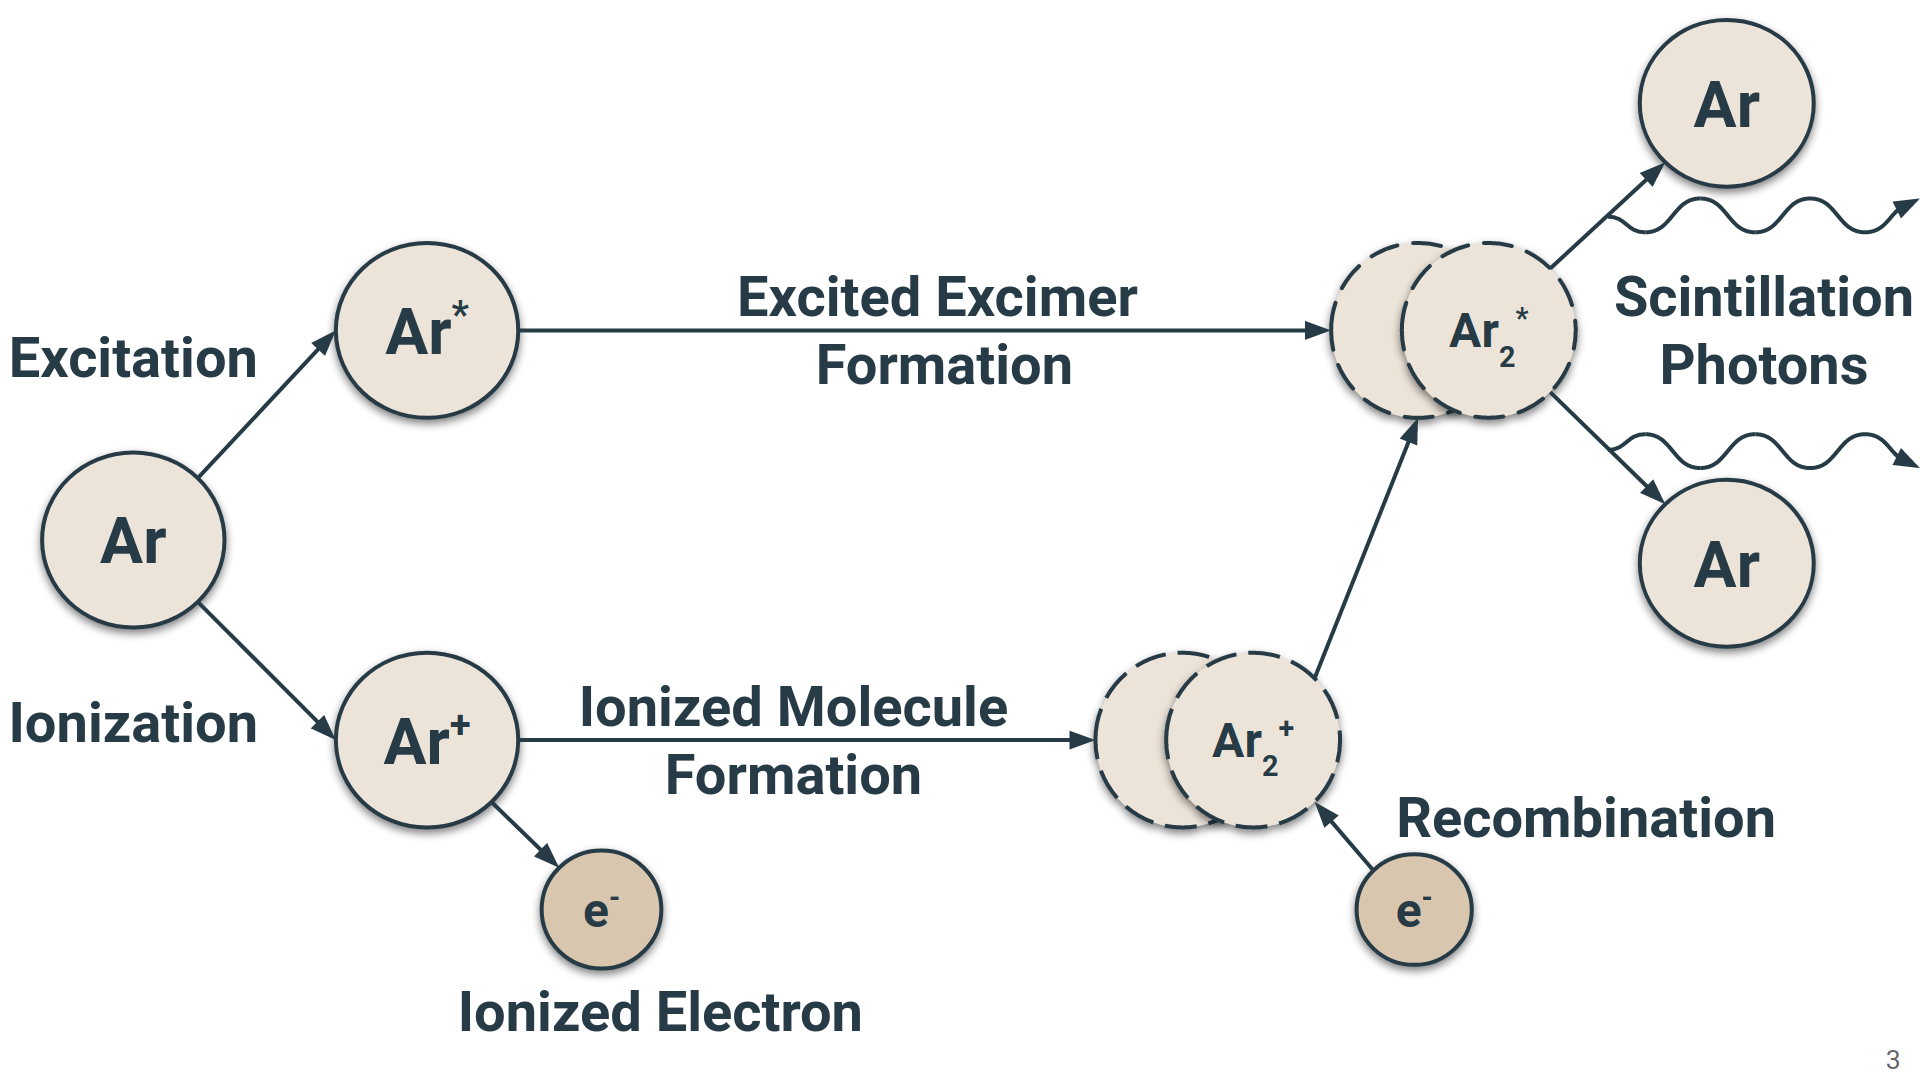
\includegraphics[width=0.6\columnwidth]{pds-lar-scintillation-schematic.png}
\end{dunefigure}

%%%%%%%%%%%%%%%%%%%%%%%%%%%%%%%%%%%%%%%%%%%%%%%%%%%%%%%%%%%+++++++++++++++++++++++++++++++++++++++++++++++++++++++++++++++++
\subsection{Design Considerations}
\label{sec:fdsp-pd-des-consid}

The principal task of the \dword{sp} \dword{pds} is to measure the \dword{vuv} scintillation light produced by ionizing tracks in the \dword{tpc} within the geometrical constraints of the \dword{apa} structure. The modular arrangement of the \dword{spmod} calls for a configuration across the width of the cryostat starting with an \dword{apa} plane against one cryostat wall, and following with \dword{apa}s and \dword{cpa}s in the order  APA-CPA-APA-CPA-APA.
The structure of the \dword{apa}, along with the imperative to maximize the active volume of \dword{lar}, precludes the use of traditional large area \dwords{pmt}.  

A solution that reduces the impact of the \dword{pds} on the active volume to zero is to place the light collector modules in the inactive space between the innermost wire planes of the \dword{apa}s. To satisfy \dword{apa} fabrication constraints and mechanical integrity, we must install the modules through slots in a (wound) \dword{apa} frame 
(see Chapter~\ref{ch:fdsp-apa}).  
%(see Chapter~\ref{ch:fdsp-apa}).  
Individual \dword{pd} modules are restricted to a profile of dimensions 
\SI{23}{mm}$\times$\SI{118}{mm}$\times$\SI{2097}{mm}.  There are ten \dword{pd} modules per \dword{apa}, equally-spaced by \SI{592}{mm}, for a total of \num{1500} per \dword{spmod}.  Of these, \num{500} are mounted in central \dword{apa} frames and must collect light from both directions (dual-face), and \num{1000} are mounted in frames  near the vessel walls and collect light from only one direction (single-face).
Figure~\ref{fig:apa-frame-pds} illustrates the baseline configuration of \dword{pd} modules and \dword{apa}s in an \dword{spmod}. 

To detect scintillation light over a large area in a compact space requires a multi-step process.  First, the \dword{vuv} scintillation photons are converted to longer wavelength by chemical wavelength shifters
\footnote{The most widely used wavelength shifter for \lar detectors is  1,1,4,4-Tetraphenyl-1,3-butadiene (\dshort{tpb}), which absorbs \dword{vuv} photons and re-emits them with a spectrum centered around \SI{420}{nm}, close to the wavelength of maximum quantum efficiency for photo-conversion in most commercial photosensors.}.
These photons are then channeled as efficiently as possible toward much smaller photosensors that produce an electrical signal. Because of the severe space constraints, these must be silicon photosensors with dimensions of just a few millimeters,  not a traditional photomultiplier.
Another requirement, distinct from most previous HEP applications of these devices, is that they must operate reliably for many years at \dword{lar} temperatures. 

\begin{dunefigure}[Arrangement of APAs in a \dshort{spmod} and position of PD modules in APA frame]{fig:apa-frame-pds}
{End-on schematic view of the active argon volume showing the four drift regions and anode-cathode plane ordering of the \dword{tpc} inside the \dword{spmod} (top). The three rows of \dword{apa}s across the width of the \dword{spmod} are two frames high and 25 frames deep. Schematic of an \dword{apa} frame (on its side) showing the ten pairs of \dword{pd} module support rails (almost vertical in figure) (bottom). Notice the five slots on the frame's side that the \dword{pd} modules fit through (top of figure). The other five slots are on the frame's opposite side, at the bottom of the figure.}
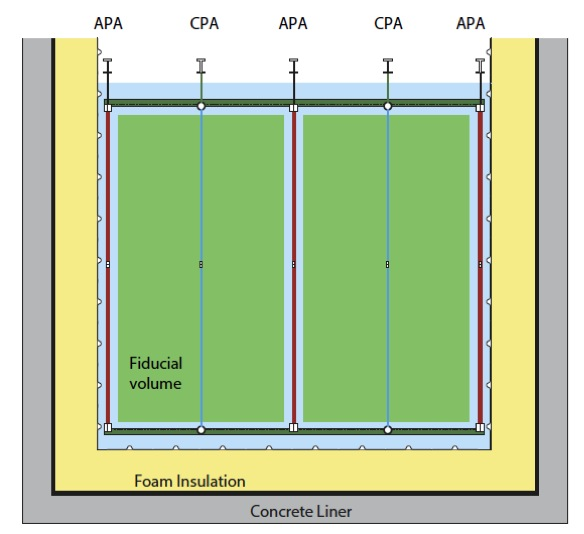
\includegraphics[width=0.6\textwidth]{sp-apa-dune-sp-end-view.jpg}
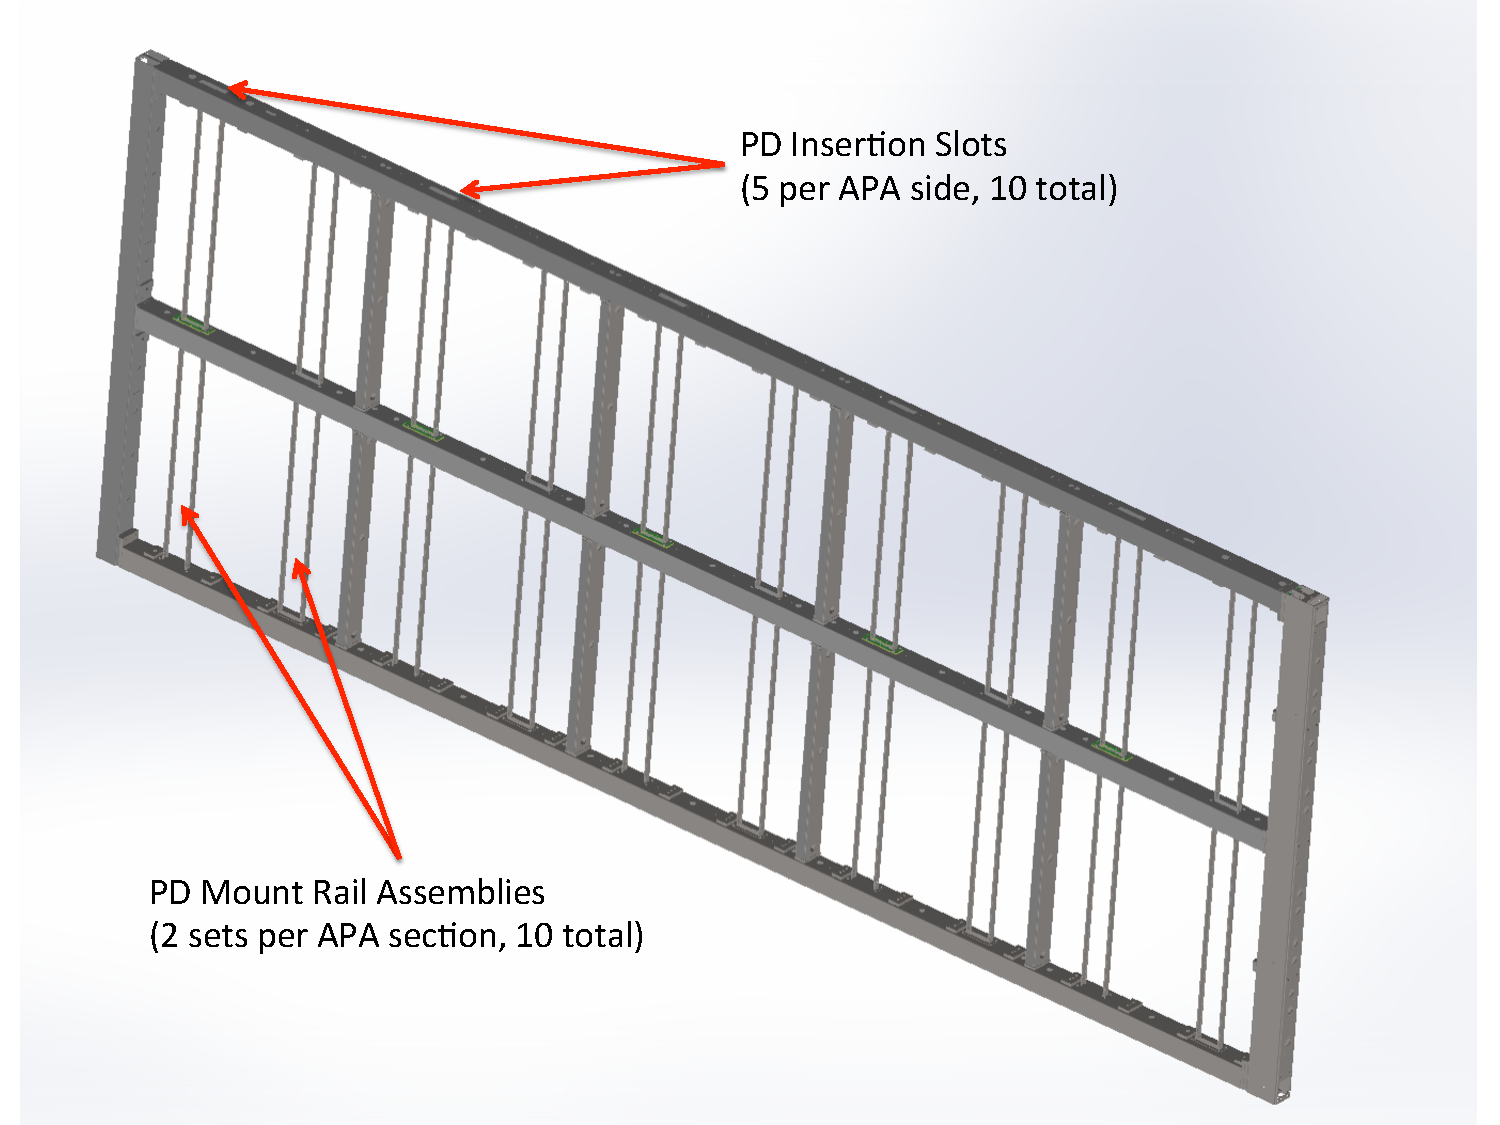
\includegraphics[width=0.8\textwidth]{pds-apa-frame-with-rails.pdf}
\end{dunefigure}

An operational consideration for the \dword{pds} design is the presence in the \dword{lartpc} of the long-lived cosmogenic radioisotope \Ar39, which has a specific activity in argon extracted from the atmosphere of approximately \SI{1}{Bq/kg}~\cite{bkds}. The isotope undergoes beta decay at a mean beta energy of \SI{220}{keV} with an endpoint of \SI{565}{keV} and makes up $\sim$70\% of the radiological background signal.
In the \SI{10}{kt} \dword{fd} modules, this leads to a rate of more than \SI{10}{MHz} of very short ($\sim$\SI{1}{mm}) tracks uniformly distributed throughout the module, each of which produces several thousand \dword{vuv} scintillation photons. This continuous background affects the \dword{daq}, trigger, and spatial granularity required of the \dword{pds}. Spatial granularity helps even more with rare but more energetic radiological backgrounds that can produce multi-photon signals, but only a single detector. Low energy neutrinos, on the other hand, will produce coincident  signals on multiple channels, allowing them to be easily identified.

%+++++++++++++++++++++++++++++++++++++++++++++++++++++++++++++++++
\subsection{Design Overview}
\label{sec:pds:des-ov}

%%% rjw 
The  large-area light collectors are the core modular elements of the \dword{pds}.  They convert incident \SI{127}{nm} scintillation photons into photons in the visible range (>\SI{400}{nm}) that compact \dword{sipm} photosensors, in turn,  convert to an electrical signal. The light collector design must optimize the costs of various components of the system while meeting the performance requirements.  Even though production cost and key performance parameters of \dwords{sipm} have improved significantly in recent years, covering the light detector surfaces with enough of them to meet the physics requirements of the \dword{pds} would be cost-prohibitive. 
The light collector design should maximize the active \dword{vuv}-sensitive area of the \dword{pds} while minimizing the necessary photocathode (\dword{sipm}) coverage. This is detailed in
Section~\ref{sec:fdsp-pd-lc}.

%%%%%%%%%%%%%%%%%%%%%
\subsubsection{Light Collectors} 
\label{sssec:photoncollectors}

\dword{dune} investigated many \dword{pd} light collector module options before forming the \dword{sp} \dword{pd} consortium; we selected four for further development. 
Two designs, \dword{sarapu}\footnote{\textit{Arapuca} is the name of a simple trap for catching birds originally used by the Guarani people of Brazil.} %(\textbf{S}tandard-) 
and \dword{xarapu}, %(e\textbf{X}tended-), 
use a relatively new scalable concept designed to provide  
significantly better performance than the other approaches. Functionally, ARAPUCA is a light trap that captures wavelength-shifted photons inside boxes with highly reflective internal surfaces until they are eventually detected by \dwords{sipm} or are lost.  The two other designs are based on the use of wavelength-shifters and long plastic light guides coupled to \dwords{sipm} at the ends. Their performance could meet the basic physics requirements but with only a small safety margin, and their performance is not easily scalable within the geometric constraints of the \dword{spmod}. 

The performance of the light collector is characterized by the \emph{collection efficiency} of the device, which is defined as the ratio of the number of detected photons and the number of \SI{127}{nm} scintillation photons incident on the light collector window.  For the ARAPUCA, this depends on three distinct aspects of the design:
\begin{itemize}
    \item The efficiency of the conversion of incident \dword{vuv} photons to photons trapped inside the cavity. This depends primarily on the wavelength shifter(s) efficiency and the fraction of converted photons that enter the cavity.
    \item The efficiency for the captured photons to eventually fall on the photosensor. This depends primarily on the reflectivity of the surfaces of the cavity, the geometry of the cavity, and the ratio of the photosensitive area to the light collector window area.
    \item The efficiency for the photosensor to convert incident photons to an electronic signal. This depends on the energy of the converted photons in the cavity and properties of the commercial sensor.
\end{itemize}
The \emph{effective area} of a \dword{pd} module is another useful figure-of-merit that is defined to be the photon collection efficiency multiplied by the photon collecting area of a \dword{pd} module. 

\textit{\dword{sarapu}:} In an \dword{sarapu} cell, enhanced photon trapping is attained when using the wavelength--shifting plates and the technology of the dichroic short-pass optical filter. These commercially available interference filters use multi-layer thin films highly transparent to photons with a wavelength below a tunable cutoff, 
with transmission typically more than 95\%, yet almost perfectly reflective to photons with a wavelength above the cutoff.  Such a filter forms the entrance window to a cell whose internal surfaces are covered by highly reflective acrylic foils
except for a small fraction occupied by \dwords{sipm}.

For the collector to act as a photon trap, the external face of the dichroic filter is coated with a wavelength shifting coating with an emission wavelength less than the cutoff wavelength of the filter. 
The transmitted photons pass through the filter where they encounter a second wavelength-shifter coated on either the inside surface of the filter plate or on the rear surface of the box.
This second wavelength-shifter has emission spectra which exceed the cutoff wavelength, thus trapping the photon inside the box.
Trapped photons reflect off the inner walls and the filter surface(s) (of reflectivity typically greater than \SI{98}{\%}) 
and have a high probability of impinging on a \dword{sipm} before being lost to absorption. 

Several iterations of the \dword{sarapu} design were tested in small cryostats (Section~\ref{sec:valid-initial}) and \dword{pdsp} (Section~\ref{sec:valid-pdsp}), establishing the viability of the concept for \dword{dune}.

\textit{\dword{xarapu}:} The \dword{xarapu}, adopted as the baseline design and detailed in 
Section~\ref{sec:fdsp-pd-lc}, is an evolution of the first generation \dword{sarapu}.  In the \dword{xarapu}, the secondary \dword{wls} layer of the \dword{sarapu} (a vacuum-deposited layer of \dword{wls} applied to the inner surfaces of the cell) is replaced by a \dword{wls} plate with an emission wavelength higher than the filter plate transmission frequency.  Wavelength shifted photons from this plate have two mechanisms for transport to the photosensors inside the cell: either they are transported along the \dword{wls} plate to the photosensors via total internal reflection, or those escaping the plate are captured due to reflection from the dichroic filter by the standard ARAPUCA effect.
The concept is illustrated in Figure~\ref{fig:arapuca}.
Validation of the \dword{xarapu} design is described in Sections~\ref{sec:xarapuca-unicamp} and \ref{sec:iceberg-teststand}.

\begin{dunefigure}[Schematic representation of the \dshort{xarapu} operating principle]{fig:arapuca}
{Schematic representation of a single-sided readout  \dword{xarapu} operating principle.  This example assumes a filter cutoff of \SI{400}{nm}. (Note: In the original ARAPUCA concept, the second wavelength-shifter was coated on the inner surface of the filter and the \dword{wls} plate shown in the figure was absent.)}               
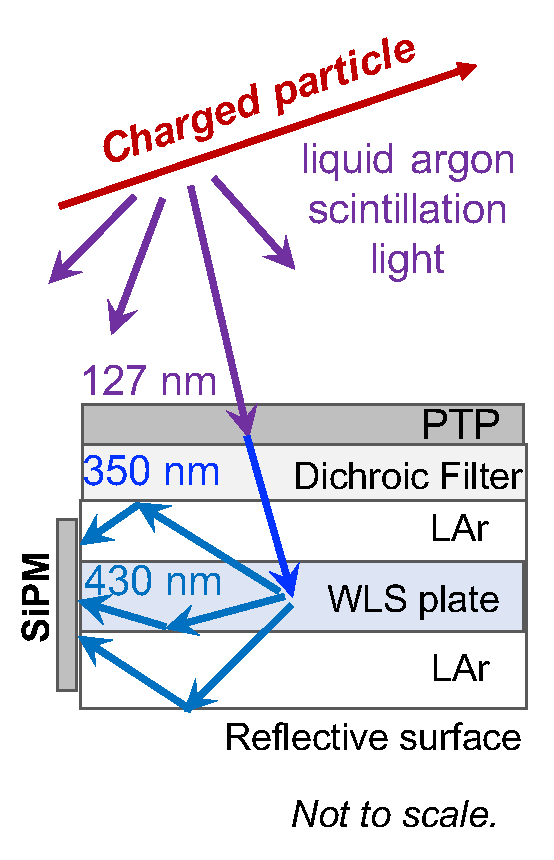
\includegraphics[height=7cm]{pds-x-arapuca-concept}   
\end{dunefigure}

While the \dword{sarapu} modules deployed in \dword{pdsp} collect light from only one direction, the next generation \dword{xarapu} can be deployed as either single-face or dual-face readout by using either an opaque reflector plate (single) or a second dichroic filter window (dual) on the second face. 
Figure~\ref{fig:3dtpc-pd} shows how a light-collector module is incorporated into an \dword{apa}. One module spans the width of an \dword{apa}. Figure~\ref{fig:pds-pd-full-module} (left) shows a detail of the module where the 24 \dword{xarapu} cells are visible on either side of a signal summing and interface board that becomes enclosed by the hollow central beam of the \dword{apa} frame. Figure~\ref{fig:pds-pd-full-module} (right) illustrates how a module is inserted into an \dword{apa} frame.


\begin{dunefigure}[\threed model of \dshorts{pd} in the \dshort{apa}]{fig:3dtpc-pd}
{\threed model of \dwords{pd} in the \dword{apa}. The model on the left shows the full width of a one \dword{apa} deep slice of the \dword{tpc} illustrating the APA-CPA-APA-CPA-APA system configuration. The figure on the right shows a detail of the top far side of the \dword{tpc} where three photon collector modules are visible.}
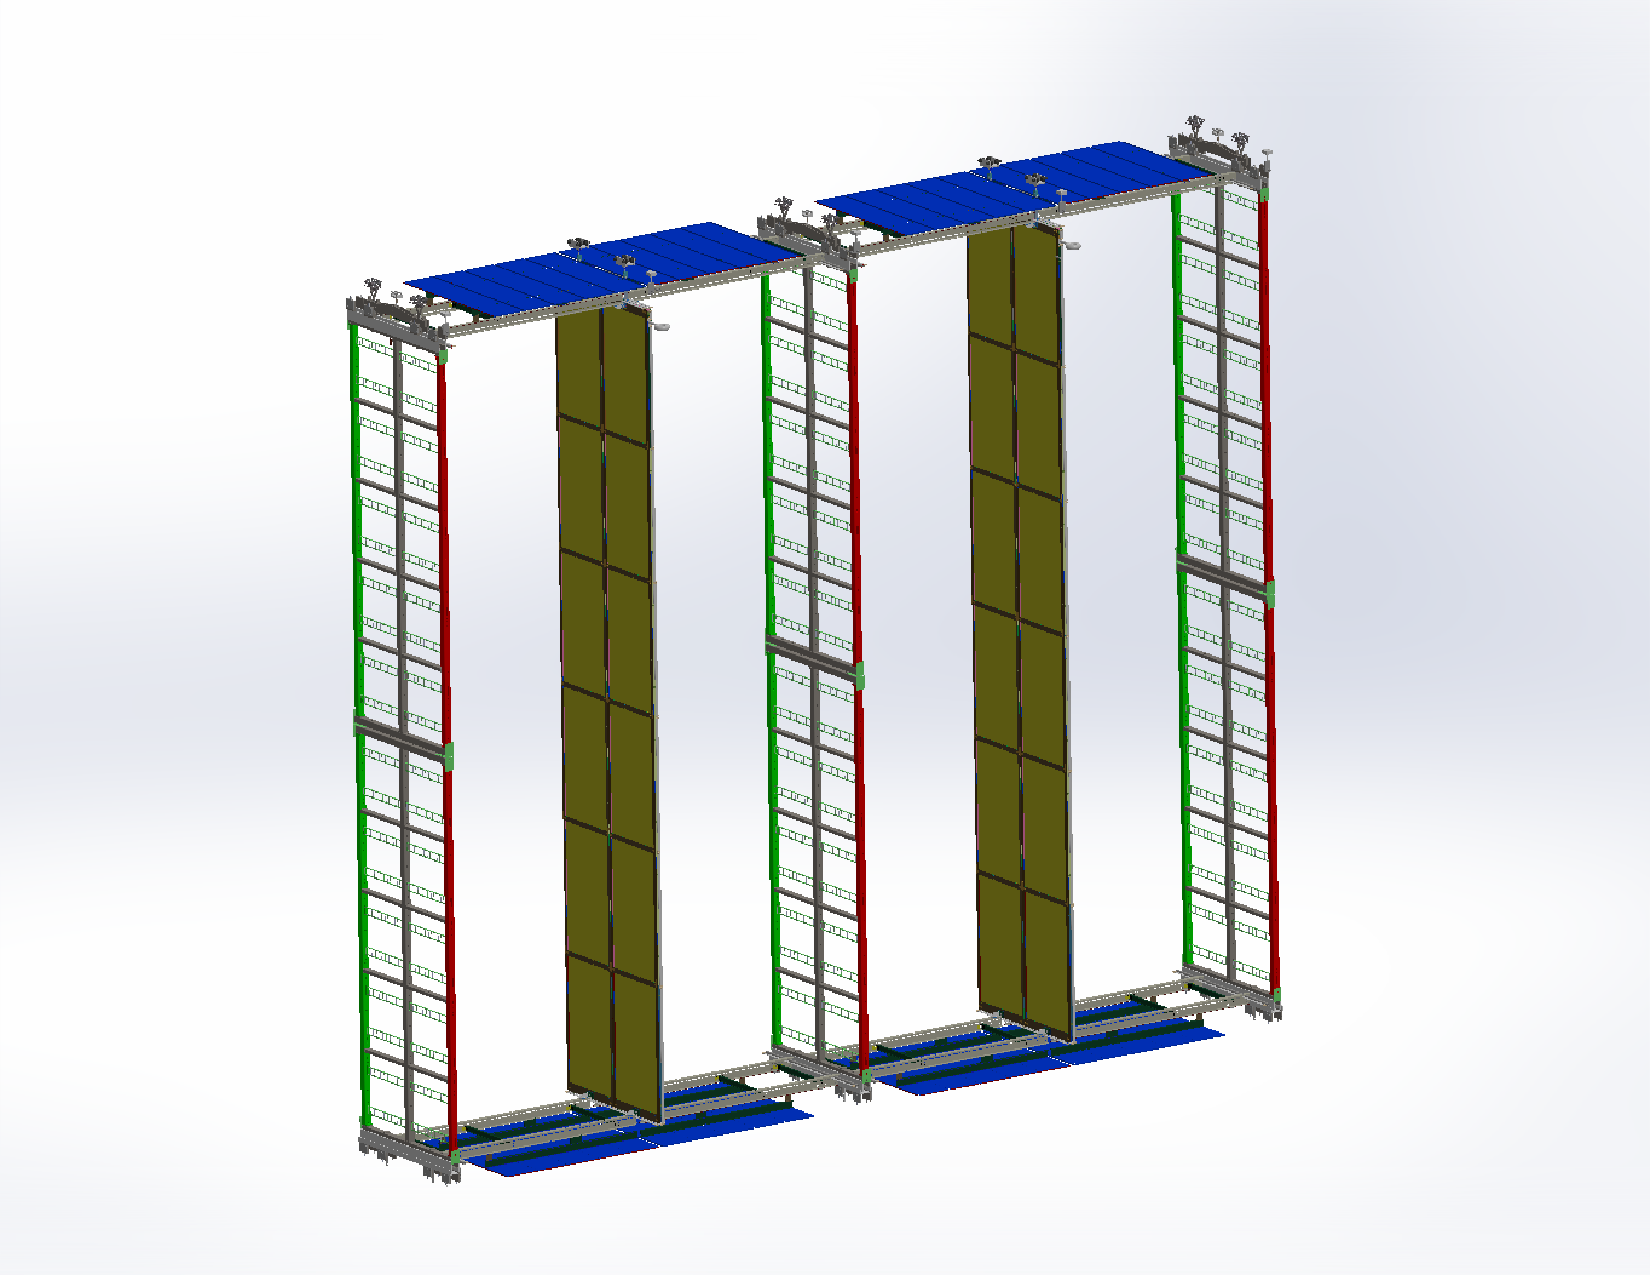
\includegraphics[height=6.5cm]{pds-apa-cpa-assembly-2}
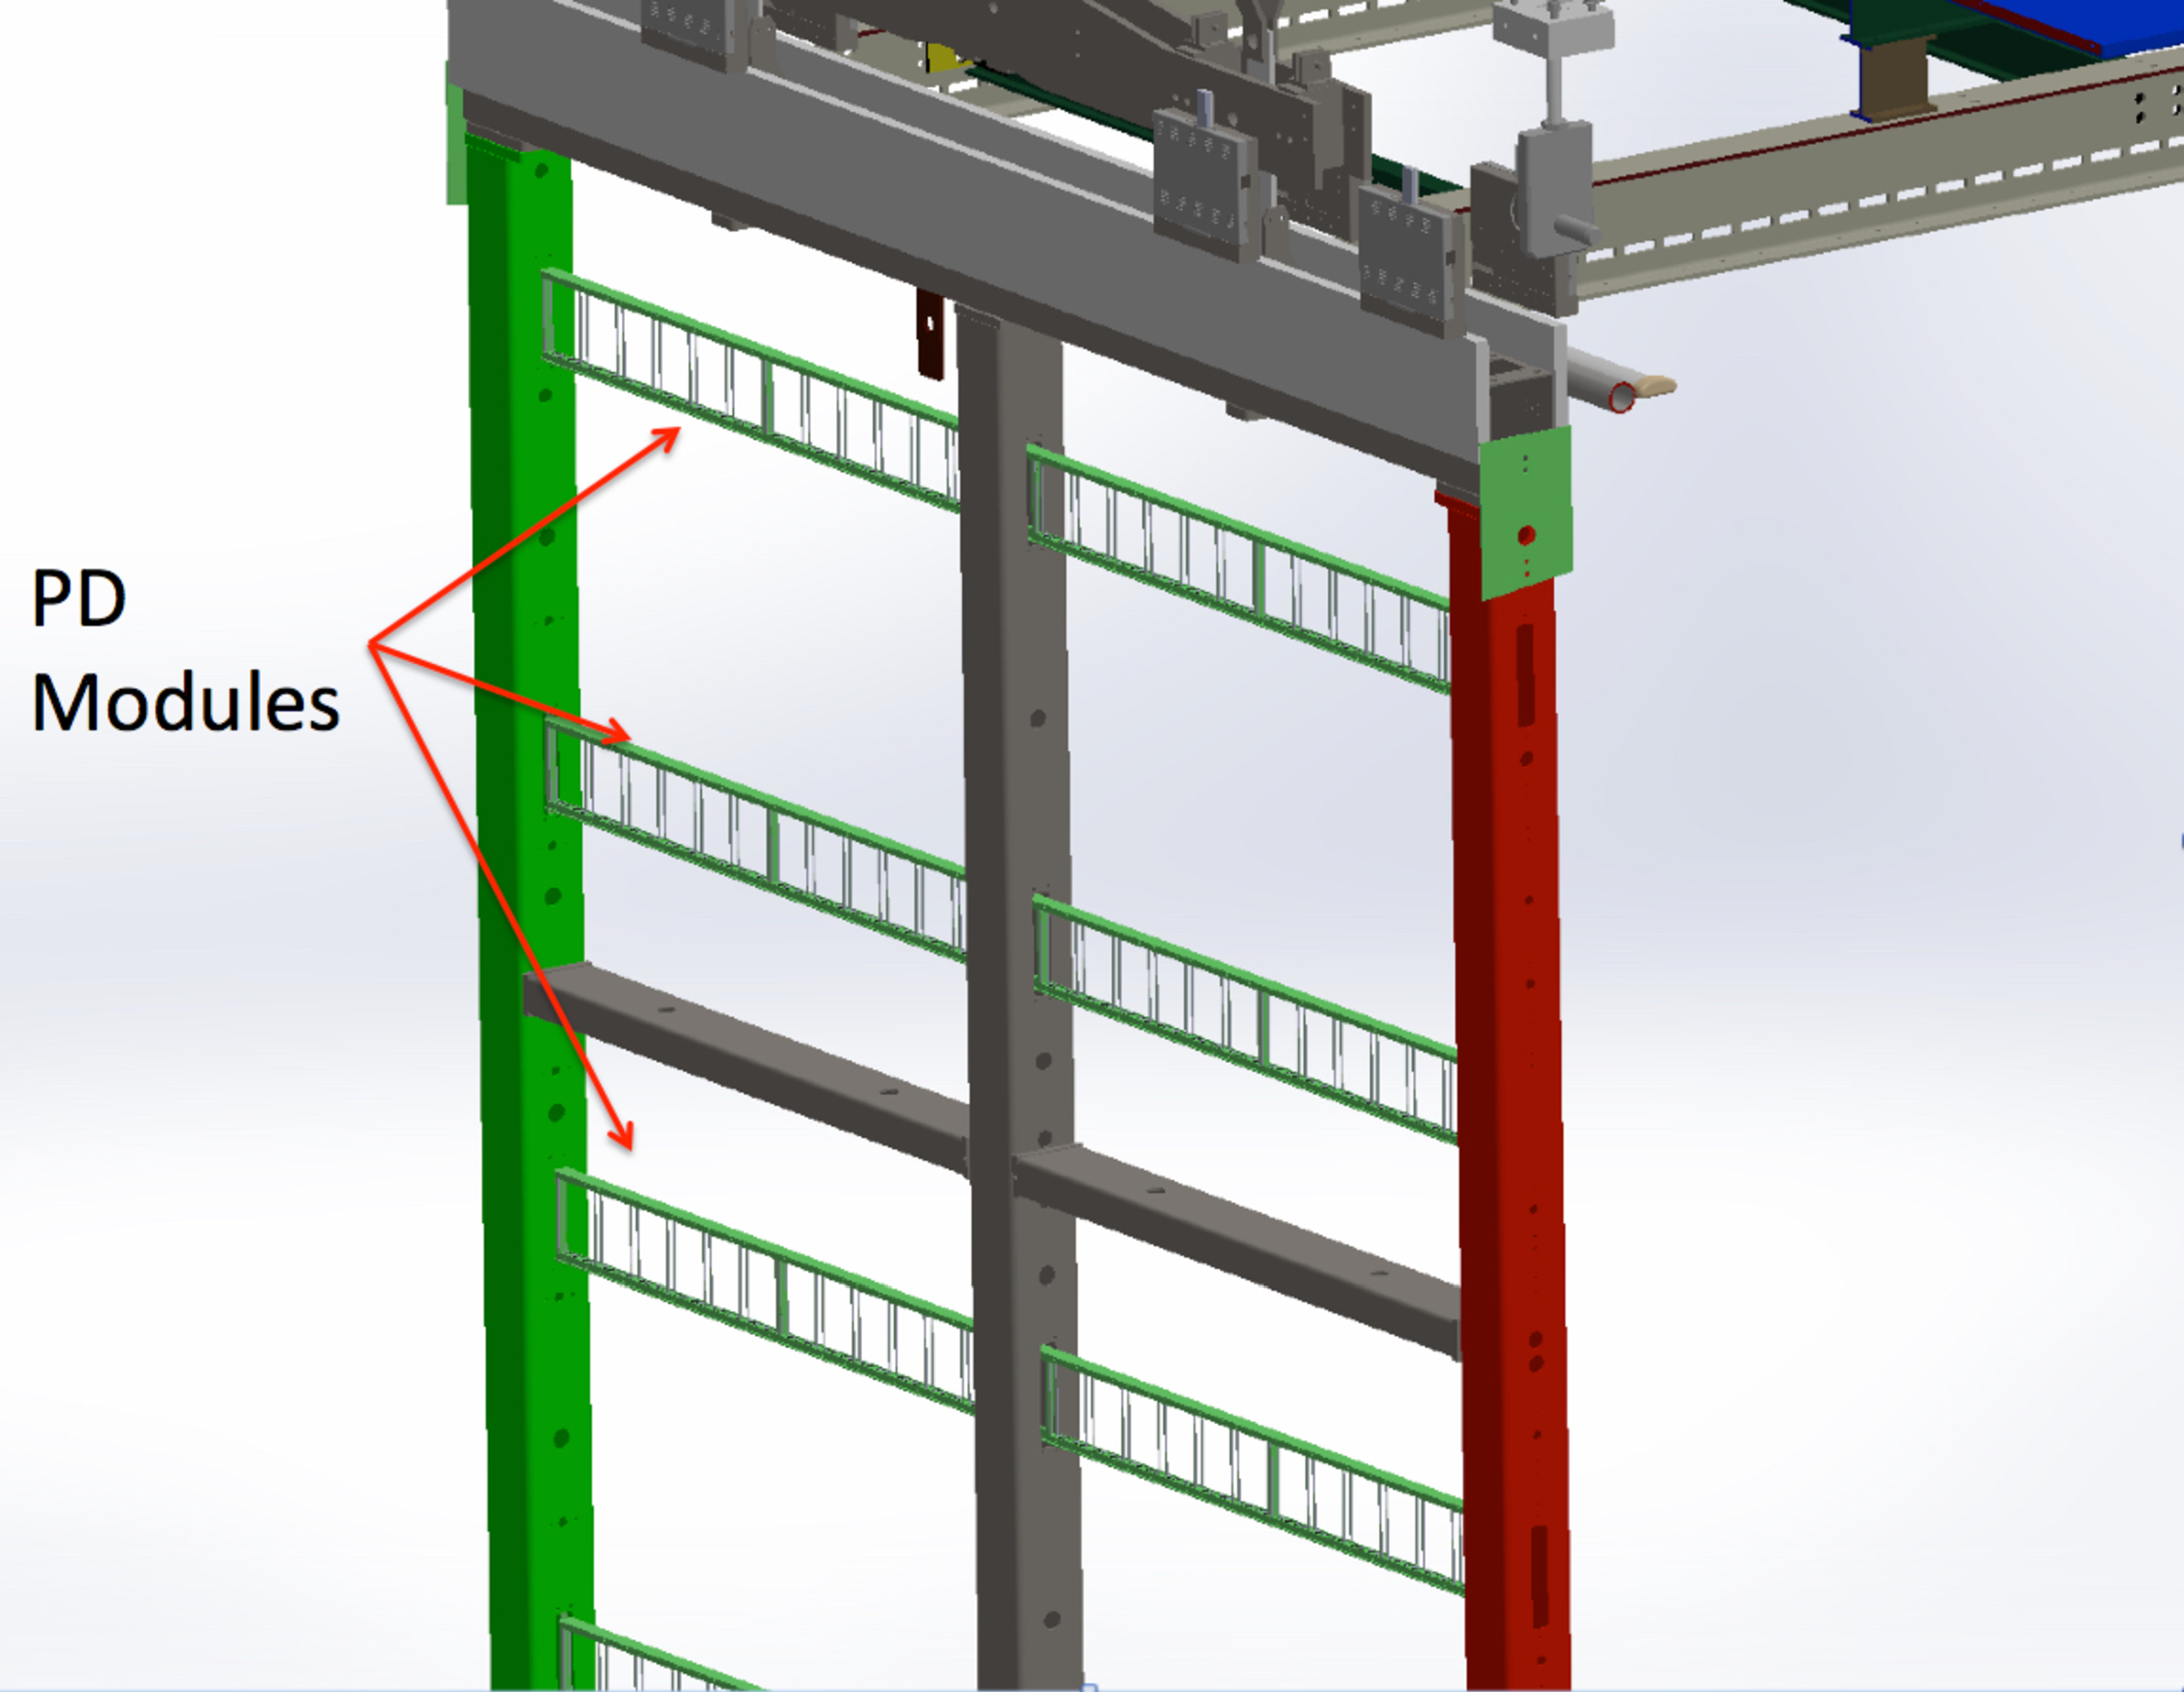
\includegraphics[height=6.5cm]{pds-pds-in-apa-assembly-r4}
\end{dunefigure}

\begin{dunefigure}[PD Module being inserted into an APA frame]{fig:pds-pd-full-module}
{Solid model of a \dword{pd} module being inserted into an \dword{apa} frame (wires not shown), which is done after the APA assembly is completed.}
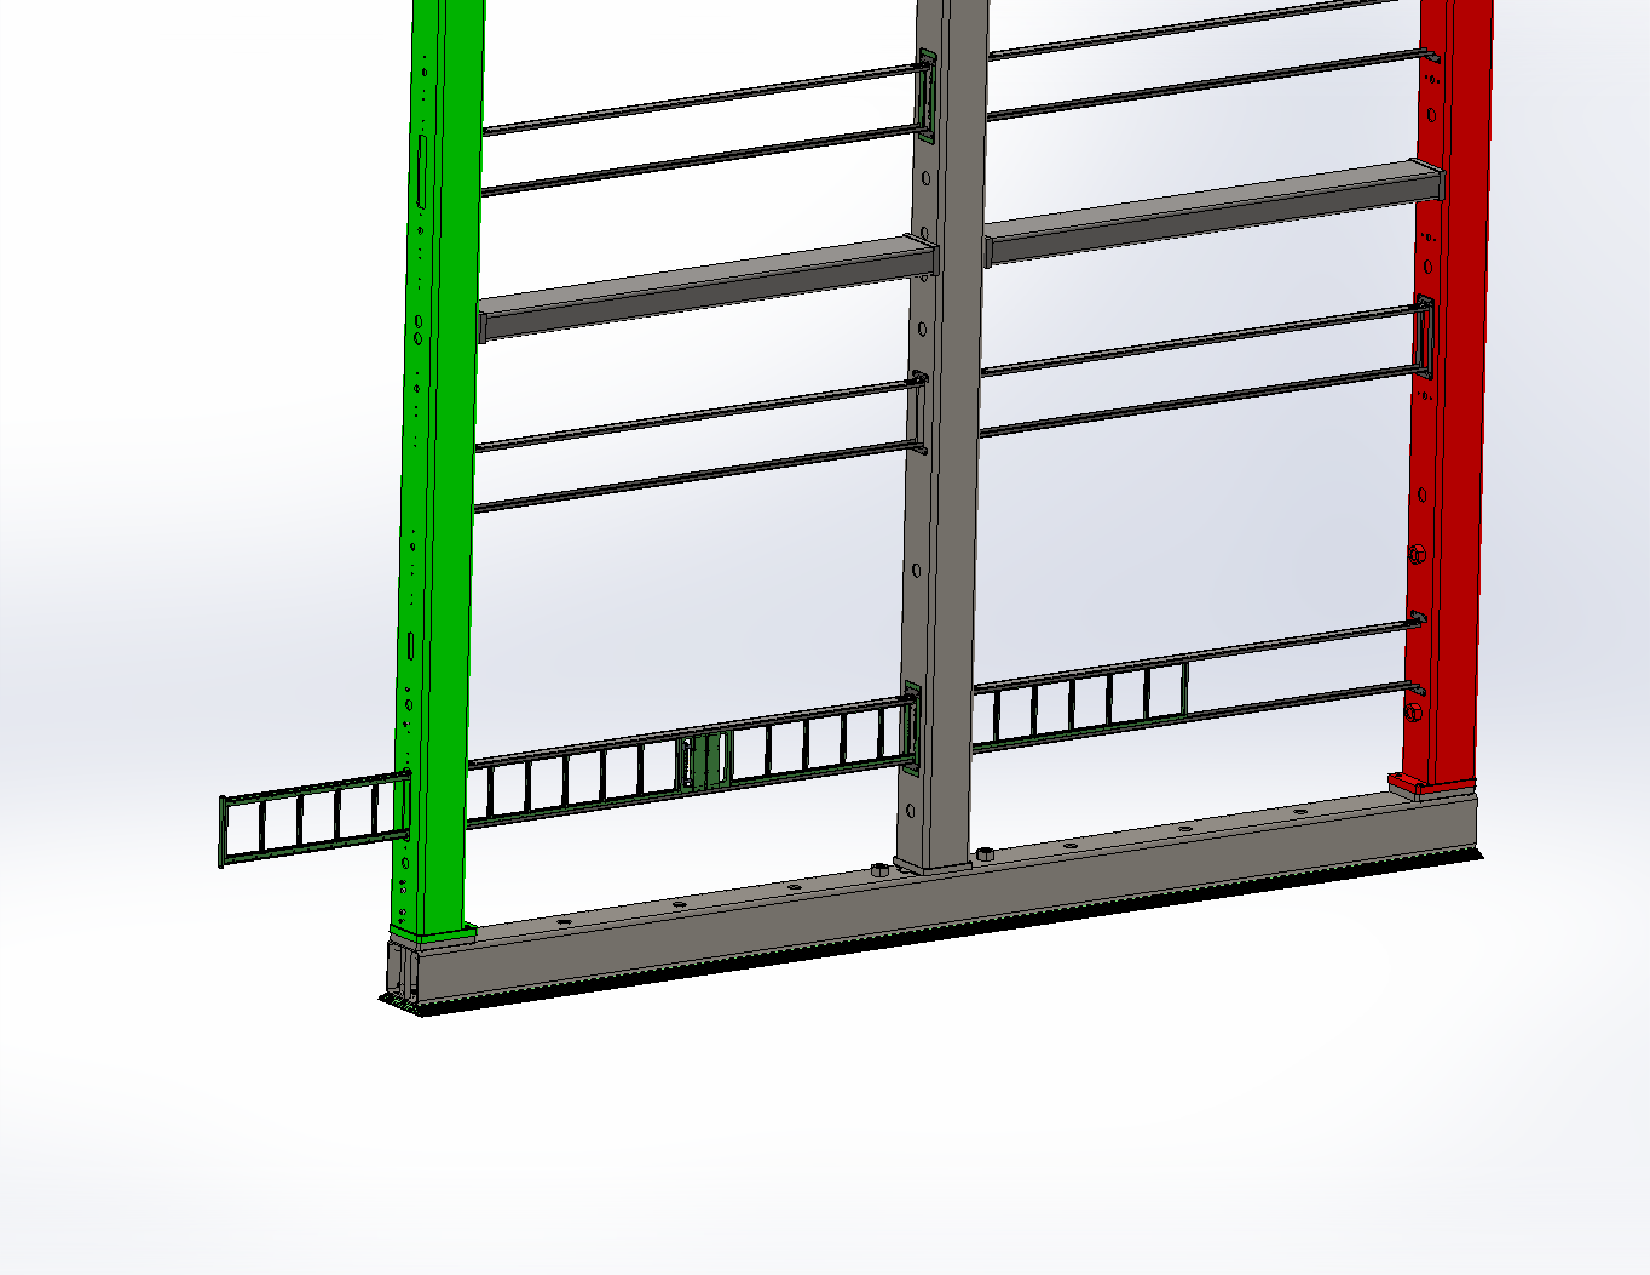
\includegraphics[height=6.5cm]{pds-pd-module-inserting-into-apa}
\end{dunefigure}

The \dword{xarapu} light collector design has the flexibility to accommodate greater demands, such as might be desired for \dword{sbn} physics, without major changes. One example of this flexibility is the ability to increase the number of \dwords{sipm} to increase light yield, which could be incorporated quite late in the final design stages because it would not involve significant mechanical changes.

%%%%%%%%%%
\subsubsection{Silicon Photosensors} 
\label{sssec:photosensors}

The \dword{sp} \dword{pds} uses a multi-step approach to scintillation light detection with the final stage of conversion into electrical charge performed by \dwords{sipm}. Robust photon conversion efficiency, low operating voltages, small size, and ruggedness make their use attractive in the \dword{sp} design where the \dwords{pd} must fit inside the \dword{apa} frames. 

Based on extensive testing and experience with the vendor, we have selected a \SI{6}{mm}$\times$\SI{6}{mm} \dword{mppc} % (Multi-Pixel Photon Counters) 
produced by Hamamatsu\footnote{Hamamatsu\texttrademark{} Photonics K.K., \url{http://www.hamamatsu.com/}.} (Japan) as the baseline \dword{sipm} device. 
We are also vigorously pursuing an alternative based on the design of a device developed for operation in \dword{lar} by the DarkSide experiment collaboration and Fondazione Bruno Kessler (FBK)\footnote{Fondazione Bruno Kessler\texttrademark{}, \url{https://www.fbk.eu}.} (Italy).

The baseline \dword{pds} design has \num{192} %\SI{6}{mm}$\times$\SI{6}{mm} 
\dwords{mppc} per \dword{pd} module with groups of \num{48} \dwords{mppc} electrically ganged into four electronics readout channels, which provides some spatial granularity within a module and helps to reduce the impact of radiological noise. This configuration has a total of \num{288000} \dwords{mppc} per \dword{spmod}. 

%%%%%%%%%%%%%%%%%%%%%%%%%%%%%%%%%%

\subsubsection{Readout Electronics} 

The \dword{pds} design requires an electronics readout system that collects and processes electric signals from photosensors in \dword{lar} to (1) provide the interface to trigger and timing systems,
and (2) enable data transfer to an offline storage system for physics analysis. The quantitative requirements for the system are driven by many \dword{fd} level specifications that affect signal size sensitivity, \dword{s/n}, timing resolution, event size and data transfer limits from the \dword{daq}, power needs and dissipation limits, channel density and channel count, and cost. 

As described in Section~\ref{sssec:photosensors}, each electronics signal from a \dword{pd} module is formed from an ensemble of 48 Hamamatsu \dwords{mppc} summed into a single channel by a combination of passive and active ganging.  A cold amplifier adjusts the \dword{mppc} output signal level before transmitting the signal over $\sim\,$\SI{20}{m} long\footnote{Cable lengths are not uniform across all \dwords{pd}, ranging from \SI{15}{m} at the shortest to \SI{27.25}{m} at the longest, averaging \SI{20}{m}.} twisted-pair cables to the input of \dword{fe} \dwords{adc} outside the cryostat.  The twisted pair cable is impedance-matched to  the receiver amplifiers for the \dwords{adc} to optimize common-mode noise rejection at the input of the front-end digitizer. 

The digitizer is a low-cost solution based on commercial ultrasound \dword{asic} chips rather than digitizers based on flash \dwords{adc} used in \dword{pdsp}. Inspiration for this \dword{fe} comes from the system developed for the \dword{mu2e} experiment \dword{crt} readout system as described in Section~\ref{sec:electronics}.

The \dword{fe} will continuously digitize the input signals for each channel and store waveforms alongside event metadata that meet the trigger conditions. In an externally triggered waveform mode, the configured waveform window at the time of the external trigger is also stored. These internally or externally triggered waveforms are transmitted to the \dword{daq} board reader processes for storage. The \dword{daq} system and data storage limitations impose constraints on the data bandwidth, readout rates, and zero suppression. 

Single \phel signals from \Ar39 and radiological backgrounds will dictate threshold level adjustments.
We will configure the photon readout to trigger on signals from the central trigger and timing systems for a variety of configurable events, e.g., beam events, cosmic
muons, periodic triggering, random triggering, or any combination of
these. A special trigger condition needed for \dword{snb} observation will enable readout of all digitized data over predefined periods.
The interface design will define the power, grounding, and rack schemes.


\subsection{Options to Improve Uniformity of Response} 

Because the \dword{pd} modules are installed only in the \dword{apa}, light collection is not uniform over the entire active volume of the \dword{tpc}. 
Though not necessary to meet the basic \dword{dune} performance specifications, improving the uniformity of the response would increase the trigger efficiency, simplify the analysis for \dword{snb} neutrinos and increase the light yield of the detector, which could enable enhanced calorimetric measurements based on light emitted by the ionizing particles.

The primary source of non-uniformity of response is that the Rayleigh scattering length for \SI{127}{nm} scintillation photons is relatively short compared to the size of the \dword{tpc} active volume.   
%As options, 
In parallel to the baseline design, we are pursuing two options that convert \SI{127}{nm} scintillation photons to longer wavelength photons that have a longer Rayleigh scattering length, significantly improving light collection uniformity:
\begin{itemize}
\item Use of a wavelength--shifter--coated cathode plane; see Appendix Section~\ref{sec:fdsp-pd-enh-cathode}.
\item Use of trace amount of xenon in the \dword{lar}; see Appendix Section~\ref{sec:fdsp-pd-enh-xenon}.
\end{itemize}


\subsection{Overview Summary} 
\label{sec:fdsp-pd-ov-summ}

As described in Sections~\ref{subsec:fdsp-pd-simphys-ndk} and~\ref{subsec:fdsp-pd-simphys-snb}, the performance required for the \dword{pds} to achieve 99\% for tagging nucleon decay events is a light yield of \SI{0.5}{PE/MeV} at the furthest point (near the \dword{cpa}), while the requirement to enable a calorimetric energy measurement with the \dword{pds} for low-energy events like \dwords{snb} is \SI{20}{PE/MeV} averaged over the active volume (FD-SP-3 in Table~\ref{tab:specs:SP-PDS}). The relationship between these two different light yields and the collection efficiency of the \dword{pds} depends on the assumed Rayleigh scattering length. Conservatively assuming that this length is \SI{60}{cm}, the \SI{0.5}{PE/MeV} at the \dword{cpa} corresponds to a collection efficiency of 1.3\% and the \SI{20}{PE/MeV} averaged over the active volume corresponds to an efficiency of 2.6\%.

Although full validation of the \dword{sp} \dword{pds} light collection system is still in progress, initial results on the \dword{xarapu} prototype are very encouraging -- the single cell prototype (Section~\ref{sec:xarapuca-unicamp}) has achieved a collection efficiency of $\SI{3.5}{\%}$.  This is significantly higher than the requirement.

A measured collection efficiency in excess of the specification ensures a safety margin against degradation in performance of the optical components over time and failures of a fraction of inaccessible active components during long term operation of the detector. It also opens broader opportunities for the photon detection system to extend the physics reach of the experiment, perhaps in unanticipated ways.

